\documentclass[border=12pt]{article}
\usepackage[dvipsnames]{xcolor}
\definecolor{unkblue}{HTML}{004D86}
\definecolor{unkgold}{HTML}{E4A115}
\usepackage{tikz}
\usepackage{utopia}
\usepackage[lining]{libertine}
\newenvironment{tightcenter}{%
  \setlength\topsep{-20pt}
  %\setlength\parskip{-20pt}
  \begin{center}
}{%
  \end{center}
}

\usetikzlibrary{shadows}

\begin{document}
\LARGE
  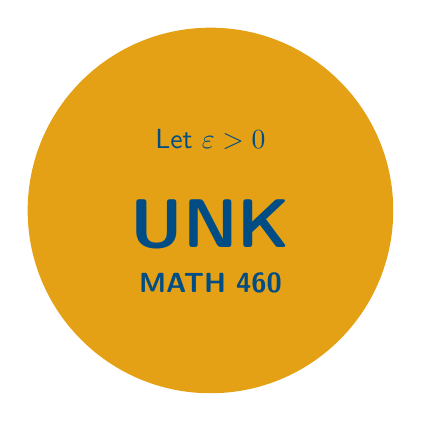
\begin{tikzpicture}
    \node[circle,minimum width=1.5in,text=unkblue,fill=unkgold,font=\sffamily] at (0,0) {  \begin{minipage}[c]{1.5in}  \begin{tightcenter}  Let \(\varepsilon  > 0 \)  \end{tightcenter}  \hfill  \\  \begin{tightcenter}  \Huge \textbf{UNK}  

 \end {tightcenter} \hfill   \\   \begin{tightcenter} \textbf{MATH 460}   \end{tightcenter} \end{minipage} };

  \end{tikzpicture}



\end{document}




